\documentclass{beamer}

% Theme
\usetheme{Madrid}
\usecolortheme{default}

% Packages
\usepackage{graphicx}
\usepackage{amsmath}
\usepackage{hyperref}
\usepackage{subcaption}
\usepackage{caption}

\usepackage{amssymb}
\usepackage{algorithm}
\usepackage{algpseudocode}
\usepackage{amsmath}

% Title information
\title[HES Denoising]{A Heuristic for Denoising Hall Effect Sensor Signals: A Case Study in Weld Current Detection}
\author{Matthew Belanger}
\institute{University of Windsor}
\date{\today}

\begin{document}

%------------------------------------------------
\begin{frame}
    \titlepage
\end{frame}

%------------------------------------------------
\begin{frame}
    \tableofcontents
\end{frame}

\section{Background}
\begin{frame}{Background}
    \begin{itemize}
        \item Signal processing involves the analysis, manipulation, and interpretation of signals \cite{ebsco_signal_processing}

        \item Signal processing enables:
        \begin{itemize}
            \item Extracting meaningful information from raw data
            \item Improving data quality
        \end{itemize}

        \item It is foundational to modern technology \cite{ebsco_signal_processing}:
        \begin{itemize}
            \item Network Communications
            \item Computer Vision
            \item Industrial and Scientific Sensing Systems
        \end{itemize}
    \end{itemize}
    \begin{figure}
        \centering
        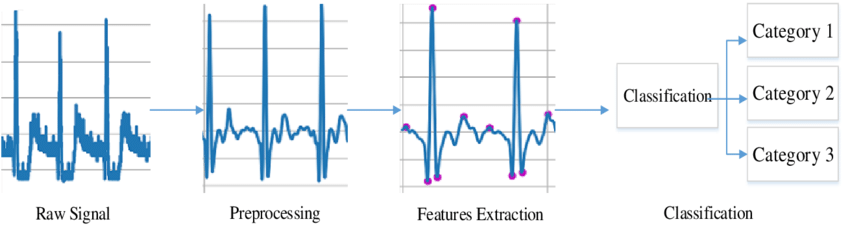
\includegraphics[width=0.9\linewidth]{images/signal-processing-system.png}
        \caption{Example Signal Processing Pipeline \cite{signal_proc_image}}
        \label{fig:sig_proc_sys}
    \end{figure}    
\end{frame}
%------------------------------------------------
\begin{frame}{Background}
    \begin{itemize}
        \item \textbf{Signals} are functions that convey information about a system \cite{Priemer1991IntroductorySignalProcessing}
        \item \textbf{Noise} is an unexpected variations in the measured signal from moment to moment or from measurement to measurement \cite{OHaver2026SignalsAndNoise}
        \item \textbf{Denoising} is then simply the process of removing noise from signals
        \item Denoising algorithms are needed to extract actionable signals from captured signals
        \item Acting on signals is made easier when the signal is filtered to reveal features clearly
    \end{itemize}
    
    \begin{figure}[ht]
        \centering
        % --- Image row ---
        \begin{minipage}[c]{0.35\linewidth}
            \centering
            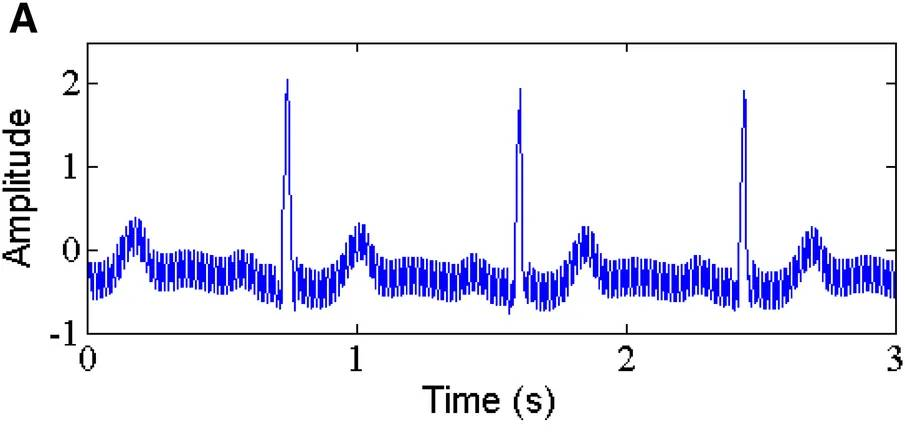
\includegraphics[width=\linewidth]{images/noisy_ecg.jpg}
        \end{minipage}
        \hspace{0.02\linewidth}
        \begin{minipage}[c]{0.05\linewidth}
            \centering
            {\LARGE\textcolor{blue}{$\Rightarrow$}}
        \end{minipage}
        \hspace{0.02\linewidth}
        \begin{minipage}[c]{0.35\linewidth}
            \centering
            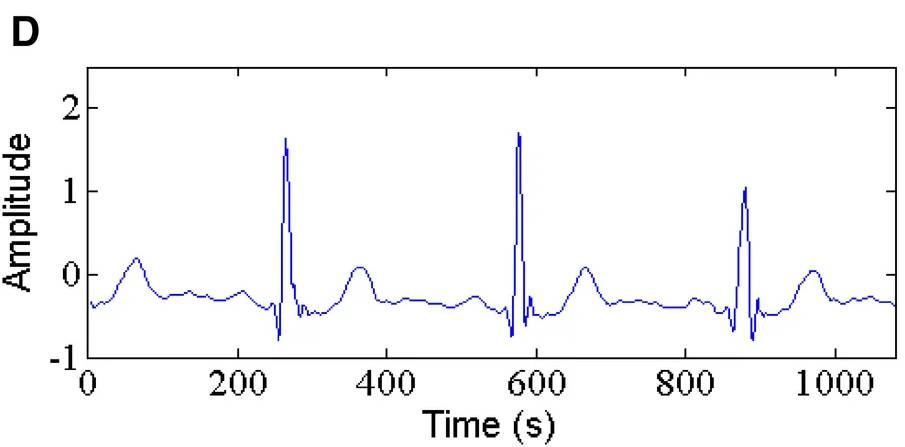
\includegraphics[width=\linewidth]{images/clean_ecg.jpg}
        \end{minipage}
    
        % --- Caption row ---
        \begin{minipage}[t]{0.35\linewidth}
            \captionof{figure}{Noisy ECG \cite{bing2024ecgdenoise}}
            \label{fig:noisy_ecg}
        \end{minipage}
        \hspace{0.09\linewidth}
        \begin{minipage}[t]{0.35\linewidth}
            \captionof{figure}{Clean ECG \cite{bing2024ecgdenoise}}
            \label{fig:clean_ecg}
        \end{minipage}
    \end{figure}
\end{frame}

%------------------------------------------------

\begin{frame}{Background}

\begin{itemize}
    \item Modern sensing systems produce continuous streams of multi-dimensional data
    \item Raw sensor measurements typically contain: \cite{OHaver2026SignalsAndNoise}
    \begin{itemize}
        \item Measurement noise
        \item Environmental interference
        \item Sensor artifacts
    \end{itemize}
    \item In signal processing pipelines, \textbf{denoising} acts as a preprocessing stage
    \item Effective preprocessing improves the performance of downstream algorithms such as \cite{Garcia2015DataPreprocessing}:
    \begin{itemize}
        \item Feature extraction
        \item Signal segmentation
        \item Machine learning models
    \end{itemize}
\end{itemize}
\begin{center}
\large
\textbf{Raw Sensor Data} $\Rightarrow$ \textbf{Signal Processing (Preprocessing)} $\Rightarrow$ \textbf{Algorithmic Decision Making}
\end{center}

\end{frame}
%----------------------------------------------------------------------------
\begin{frame}{Background}

We can interpret signals as a superposition of $K$ identifiable sources and residual random noise \cite{oppenheim1997signals}:
\[
\mathbf{Y}(n) = \sum_{i=1}^{K} \mathbf{X}_i(n) + \mathbf{N}(n)
\]
where, $\mathbf{X}_i(n)$ represents the contribution signal from the $i$-th source, and $\mathbf{N}(n)$ denotes residual noise signal not attributable to any identifiable source

Our goal is to recover the signal of the target source at sample index $n$, defined as:
\[
\hat{\mathbf{Y}}(n) = \mathbf{X}_{i^*}(n)
\]
where $i^* \in \{1, \ldots, K\}$ is the index of the target source

\end{frame}

%------------------------------------------------
\section{Literature Review}
\begin{frame}{Existing Solutions}
Solutions to this problem can be broken down into two categories:

\begin{enumerate}
    \item Denoising approaches
    \begin{itemize}
        \item Attempts to extract the prominent signal and filter out the rest
        \item Finds only $\hat{\mathbf{Y}}(n)$
    \end{itemize}
    \item Blind Source Separation (BSS)
    \begin{itemize}
        \item Attempts to assign signal components to a collection of sources, the number of which is not know a priori
        \item Finds each of $\mathbf{X}_i(n)$
        \item $\hat{\mathbf{Y}}(n)$ is the most prominent $\mathbf{X}_i(n)$
    \end{itemize}
\end{enumerate}

\end{frame}

%------------------------------------------------
\begin{frame}{Denoising Approaches: Conventional Methods}
    \begin{itemize}
        \item Khandekar \textit{et al.} conducted a comparative analysis of conventional denoising methods and modern deep learning approaches~\cite{Khandekar2025ECGDF}
        \item Found that \textbf{traditional denoising} approaches:
        \begin{itemize}
            \item $\checkmark$ Are lightweight and easy to implement
            \item $\checkmark$ Are suitable for resource-constrained environments
            \item $\times$ Have performance degradations when noise is multi-source or unpredictable
        \end{itemize}
        \item Traditional approaches include:
        \begin{itemize}
            \item Wavelet Transform 
            \item Adaptive Filtering
            \item Empirical Mode Decomposition (EMD) 
        \end{itemize}
    \end{itemize}
\end{frame}
%------------------------------------------------
\begin{frame}{Denoising Approaches: Deep Learning Methods}
    \begin{itemize}
        \item Khandekar \textit{et al.} conducted a comparative analysis of conventional denoising methods and modern deep learning approaches~\cite{Khandekar2025ECGDF}
        \item Found that advanced \textbf{deep learning} approaches:
        \begin{itemize}
            \item $\checkmark$ Strong performance in preserving signal fidelity under challenging conditions
            \item $\times$ Require large training datasets
            \item $\times$ Higher computational cost and need careful fine tuning
        \end{itemize}
        \item Some deep learning approaches considered were SOTA implementations of:
        \begin{itemize}
            \item Convolutional Neural Networks (CNN) \cite{residualcnn}
            \item Autoencoders  \cite{Zhang2025VMDRLS}
            \item Generative Adversarial Networks (GAN) \cite{Zhang2025VMDRLS}
            \item Transformers \cite{Mvuh2024MultichannelECGDenoising}
        \end{itemize}
    \end{itemize}
\end{frame}

%-------------------------------------------------
\begin{frame}{Denoising Approaches: Best Options}
    \begin{itemize}
        \item Khandekar concluded that the best performing method was CNN \cite{residualcnn} and EMD \cite{LI2025109818} was the best traditional method \cite{Khandekar2025ECGDF} 
        \begin{table}[T]
            \caption{CNN vs EMD on MIT-BIH Arrhythmia Dataset \cite{moody2001mitdb}\cite{Khandekar2025ECGDF}}
            \label{tab:ecg_comparison}
            \begin{tabular}{c c c c c}
                \hline
                \textbf{Record} & \textbf{Method} & \textbf{SNR (dB)} & \textbf{PRD (\%)} & \textbf{RMSE} \\
                \hline
                100 & CNN & 13.92 & 5.34 & 0.073 \\
                    & EMD & 11.65 & 7.89 & 0.098 \\
                \hline
                101 & CNN & 13.75 & 5.59 & 0.076 \\
                    & EMD & 11.21 & 8.45 & 0.104 \\
                \hline
                102 & CNN & 14.10 & 5.02 & 0.070 \\
                    & EMD & 11.89 & 7.72 & 0.095 \\
                \hline
                103 & CNN & 14.23 & 4.91 & 0.068 \\
                    & EMD & 11.74 & 7.95 & 0.097 \\
                \hline
                \end{tabular}
            \end{table}
    \end{itemize}
\end{frame}

%-------------------------------------------------
\begin{frame}{Denoising Approaches: Computational Speed}
    \begin{itemize}
        \item Khandekar notes that EMD approaches are generally have slow processing \cite{Khandekar2025ECGDF}
        \item They note in their comparison that LMS Adaptive Filtering is quick and computationally efficient.
        \item Sharma \textit{et al.} applied an LMS filter to denoise an Mother and Embryo ECG signal \cite{sharma}
        \item Salah \textit{et al.} integrated an LMS filter into an FPGA ECG device which has significant computational restrictions \cite{salah}
    \end{itemize}

    \begin{figure}
        \centering
        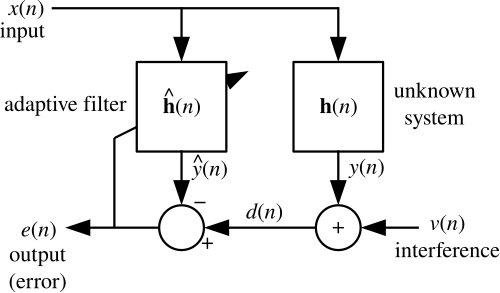
\includegraphics[width=0.35\linewidth]{images/adaptive_filter.png}
        \caption{LMS Adaptive Filter Diagram \cite{lms_filter_svg}}
        \label{fig:lms_filter}
    \end{figure}
\end{frame}
%------------------------------------------------
%\subsection{Blind Source Seperation}

\begin{frame}{Blind Source Separation}
    \begin{itemize}
        \item Hu \textit{et al.} developed a real-time approach for voice separation based on FastICA \cite{Hu2025FactoryBS}
        \item Processes data 256 samples at a time
        \item Achieves real-time BSS, assumes high speed data acquisition (8kHz)
        \item However, the processing is in addition to acquisition time making it less suitable for slower data acquisition devices
        \item Test performed on TMS320F28335 DSP platform
    \end{itemize}
    \begin{table}[htbp]
        \centering
        \caption{Real-Time Performance on DSP Platform \cite{Hu2025FactoryBS}}
        \label{tab:dsp_performance}
        \begin{tabular}{|l|l|l|}
            \hline
            \textbf{Performance Indicator} & \textbf{Value} & \textbf{Description} \\ \hline
            Single-Frame Processing Time & 25.3 ms & 256 sampling points @ 8 kHz \\ \hline
            CPU Utilization & 63.2\% & 150 MHz main frequency \\ \hline
            Memory Occupancy & 42.8 KB & SARAM + SDRAM \\ \hline
            Power Consumption & 1.8 W & Core + Peripherals \\ \hline
        \end{tabular}
    \end{table}
\end{frame}
%------------------------------------------------

\begin{frame}{Gap Analysis}
    \begin{itemize}
        \item Denoising approaches process the entire signal which does not allow us to stream the data in real time
        \item Solutions for BSS were developed for audio signals which:
        \begin{enumerate}
            \item Have high sampling rates allowing making large frame sizes feasible
            \item Latency requirements are based on the human ear which could be too slow for other applications
        \end{enumerate}
        \item Real-time solutions are rare and are tuned for specific problem domains
    \end{itemize}
\end{frame}
%------------------------------------------------

\section{Motivation}
\begin{frame}{Research Motivation}
    \begin{itemize}
        \item Resistance Spot Welding (RSW) is the most used welding method \cite{met14020185}
        \item Weld inspection after solidification only can view the final result
        \item Inline process monitoring is a promising route to zero defect manufacturing \cite{Tusinean2024}
        \item Real-time non-destructive process monitoring enables \cite{Tusinean2024}:
        \begin{itemize}
            \item Quick defect detection
            \item Improved quality control, through adaptive welding
            \item Reduced rework and scrap
        \end{itemize}
    \end{itemize}

    \begin{figure}
        \centering
        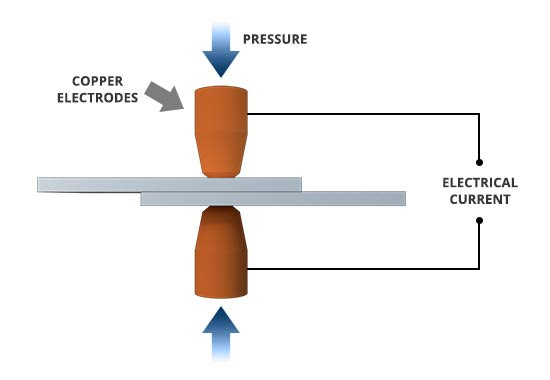
\includegraphics[width=0.35\linewidth]{images/spot-welding-diagram.jpg}
        \caption{Resistance Spot Weld Diagram \cite{TBWS2026resistance}}
        \label{fig:rsw_diagram}
    \end{figure}
\end{frame}

%------------------------------------------------
\begin{frame}{Ultrasonic Process Monitoring Equipment (UPME)}
    \begin{itemize}
        \item Provides insight into the welding process as it occurs \cite{Tusinean2024}
        \item Can identify defective welds and process deviations \cite{Tusinean2024}
        \item Can be integrated into existing manufacturing settings \cite{Tusinean2024}
        \item They are capable of:
        \begin{itemize}
            \item Fully automated operation
            \item Long-term data logging and reporting
            \item Cost-effective monitoring without human operators
        \end{itemize}
    \end{itemize}
\end{frame}

%------------------------------------------------

\begin{frame}{Challenges in Industrial Integration}
    \begin{itemize}
        \item Automotive body production requires:
        \begin{itemize}
            \item High speed
            \item High reliability
            \item Minimal human intervention
            \item Minimal customer integration support
        \end{itemize}
        \item Full automation requires:
        \begin{itemize}
            % \item Automatic sensor configuration
            \item Robust welding event detection
        \end{itemize}
        \item Existing solutions require deep integration with factory equipment
        \item High development and deployment costs
    \end{itemize}
\end{frame}

%------------------------------------------------
% \begin{frame}{Key Components of UPME}
%     \begin{itemize}
%         \item Current detection mechanism
%         \begin{itemize}
%             \item Synchronizes ultrasonic measurements with welding events
%         \end{itemize}
%         \item Ultrasonic probe configuration
%         \begin{itemize}
%             \item Determines region of interest (ROI) in time-domain signals
%         \end{itemize}
%     \end{itemize}
% \end{frame}
%------------------------------------------------

\section{Case Study: Hall Effect Sensor Based Current Detection}

\begin{frame}{Reducing Factory Interface Complexity}
    \begin{itemize}
        \item Industry efforts have been made to minimize the interface area between UPME and factory equipment
        \item I intend to detect welding current on and off events by indirectly measuring magnetic field using Hall Effect Sensors (HES)
        \item Advantages:
        \begin{itemize}
            \item No electrical connection to welding gun
            \item Reduced integration overhead
            \item Requires no signals to be provided directly by the factory 
        \end{itemize}
    \end{itemize}
\end{frame}

%------------------------------------------------
\begin{frame}{Challenges with Hall Effect Sensors}
    \begin{columns}
        \begin{column}{0.4\textwidth}
            \begin{itemize}
                \item Manufacturing environments contain many RSW guns
                \item Magnetic interference (noise) from nearby welders
                \item Modern welding schedules use:
                \begin{itemize}
                    \item Multi-impulse
                    \item Complex current profiles
                    \item Require robust signal processing
                \end{itemize}
                \item Defining a single current signature is impractical
            \end{itemize}
        \end{column}
        \begin{column}{0.6\textwidth}
            \centering
            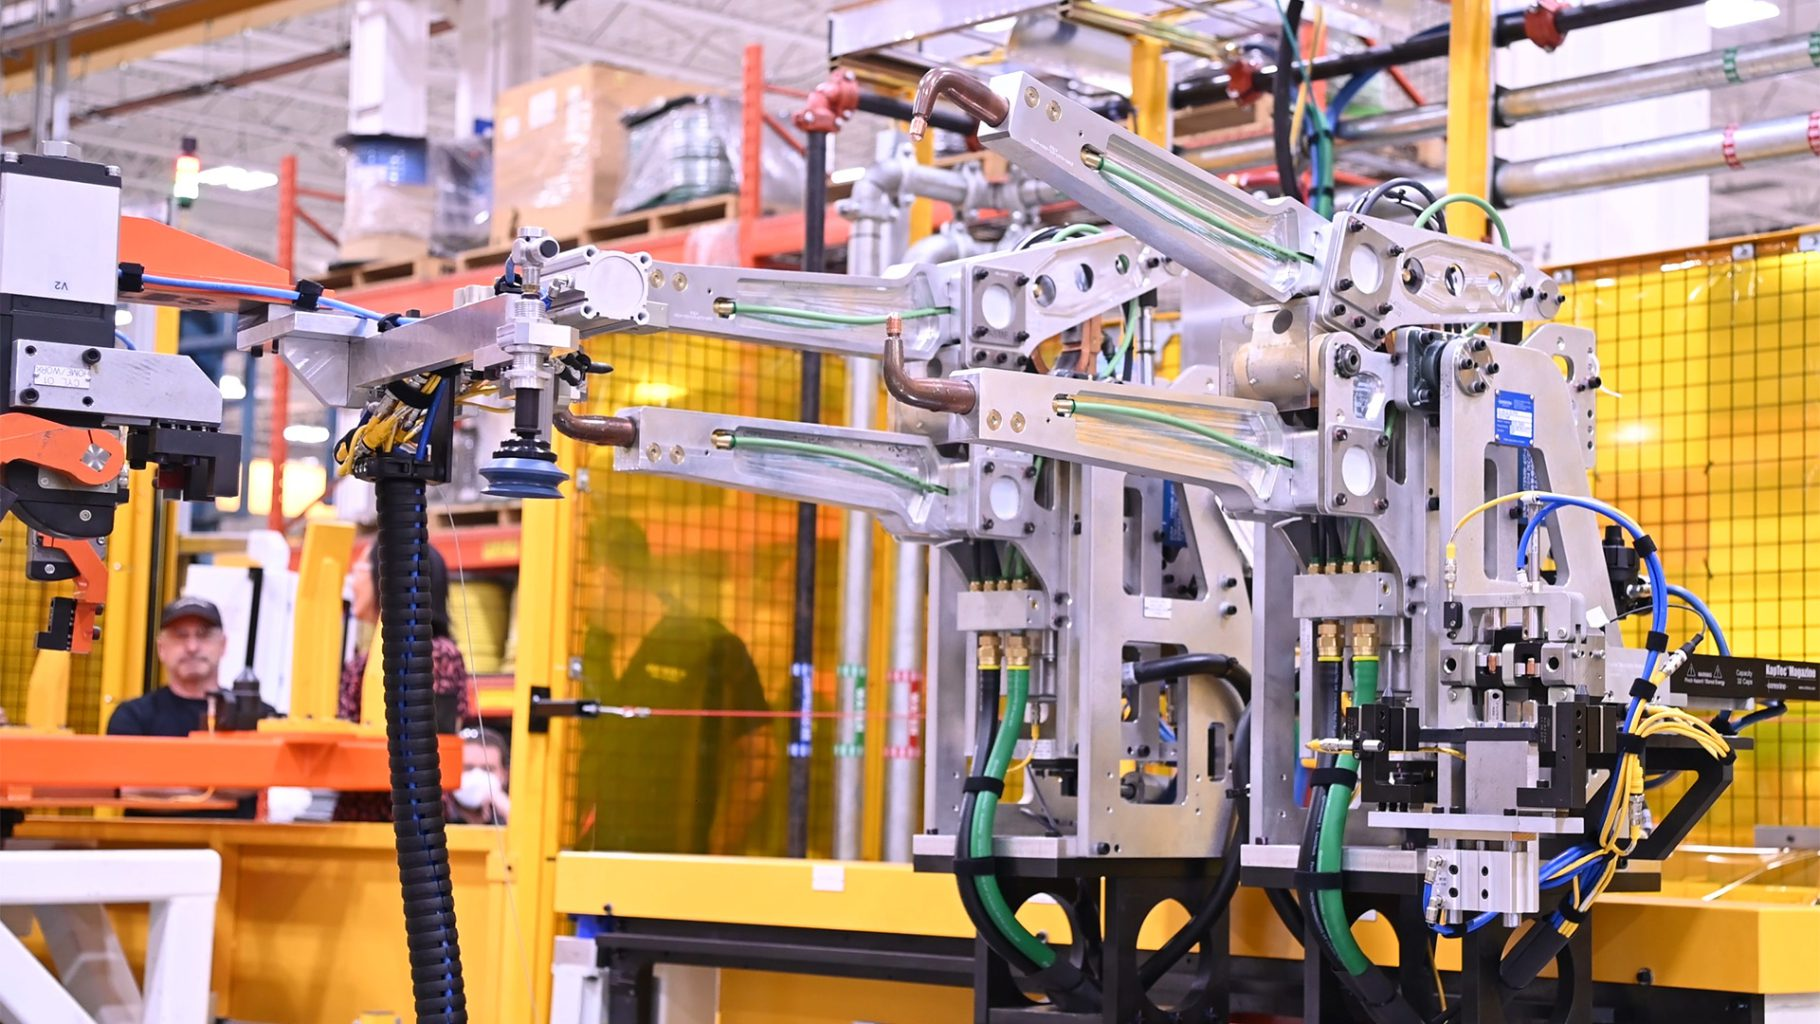
\includegraphics[width=\linewidth]{images/spot_welders.jpg}
            \captionof{figure}{Proximate RSW Guns \cite{centerline_spot_welding}}
        \end{column}

    \end{columns}
\end{frame}

%------------------------------------------------
\begin{frame}{Research Objectives: HES Signals}
    \begin{columns}
        % Left column (text)
        \begin{column}{0.55\textwidth}
            \begin{itemize}
                \item Analyze real HES signatures from different welding schedules
                \item Simulate interference from multiple welding guns
                \item Generate realistic synthetic datasets
                \item Develop algorithms to:
                \begin{enumerate}
                    \item Filter out Hall Effect signal interference
                    \item Detect current on/off events robustly from denoised signal
                \end{enumerate}
            \end{itemize}
        \end{column}
        
        % Right column (images)
        \begin{column}{0.45\textwidth}
            \begin{figure}
                \centering
                \begin{subfigure}{0.48\textwidth}
                    \centering
                    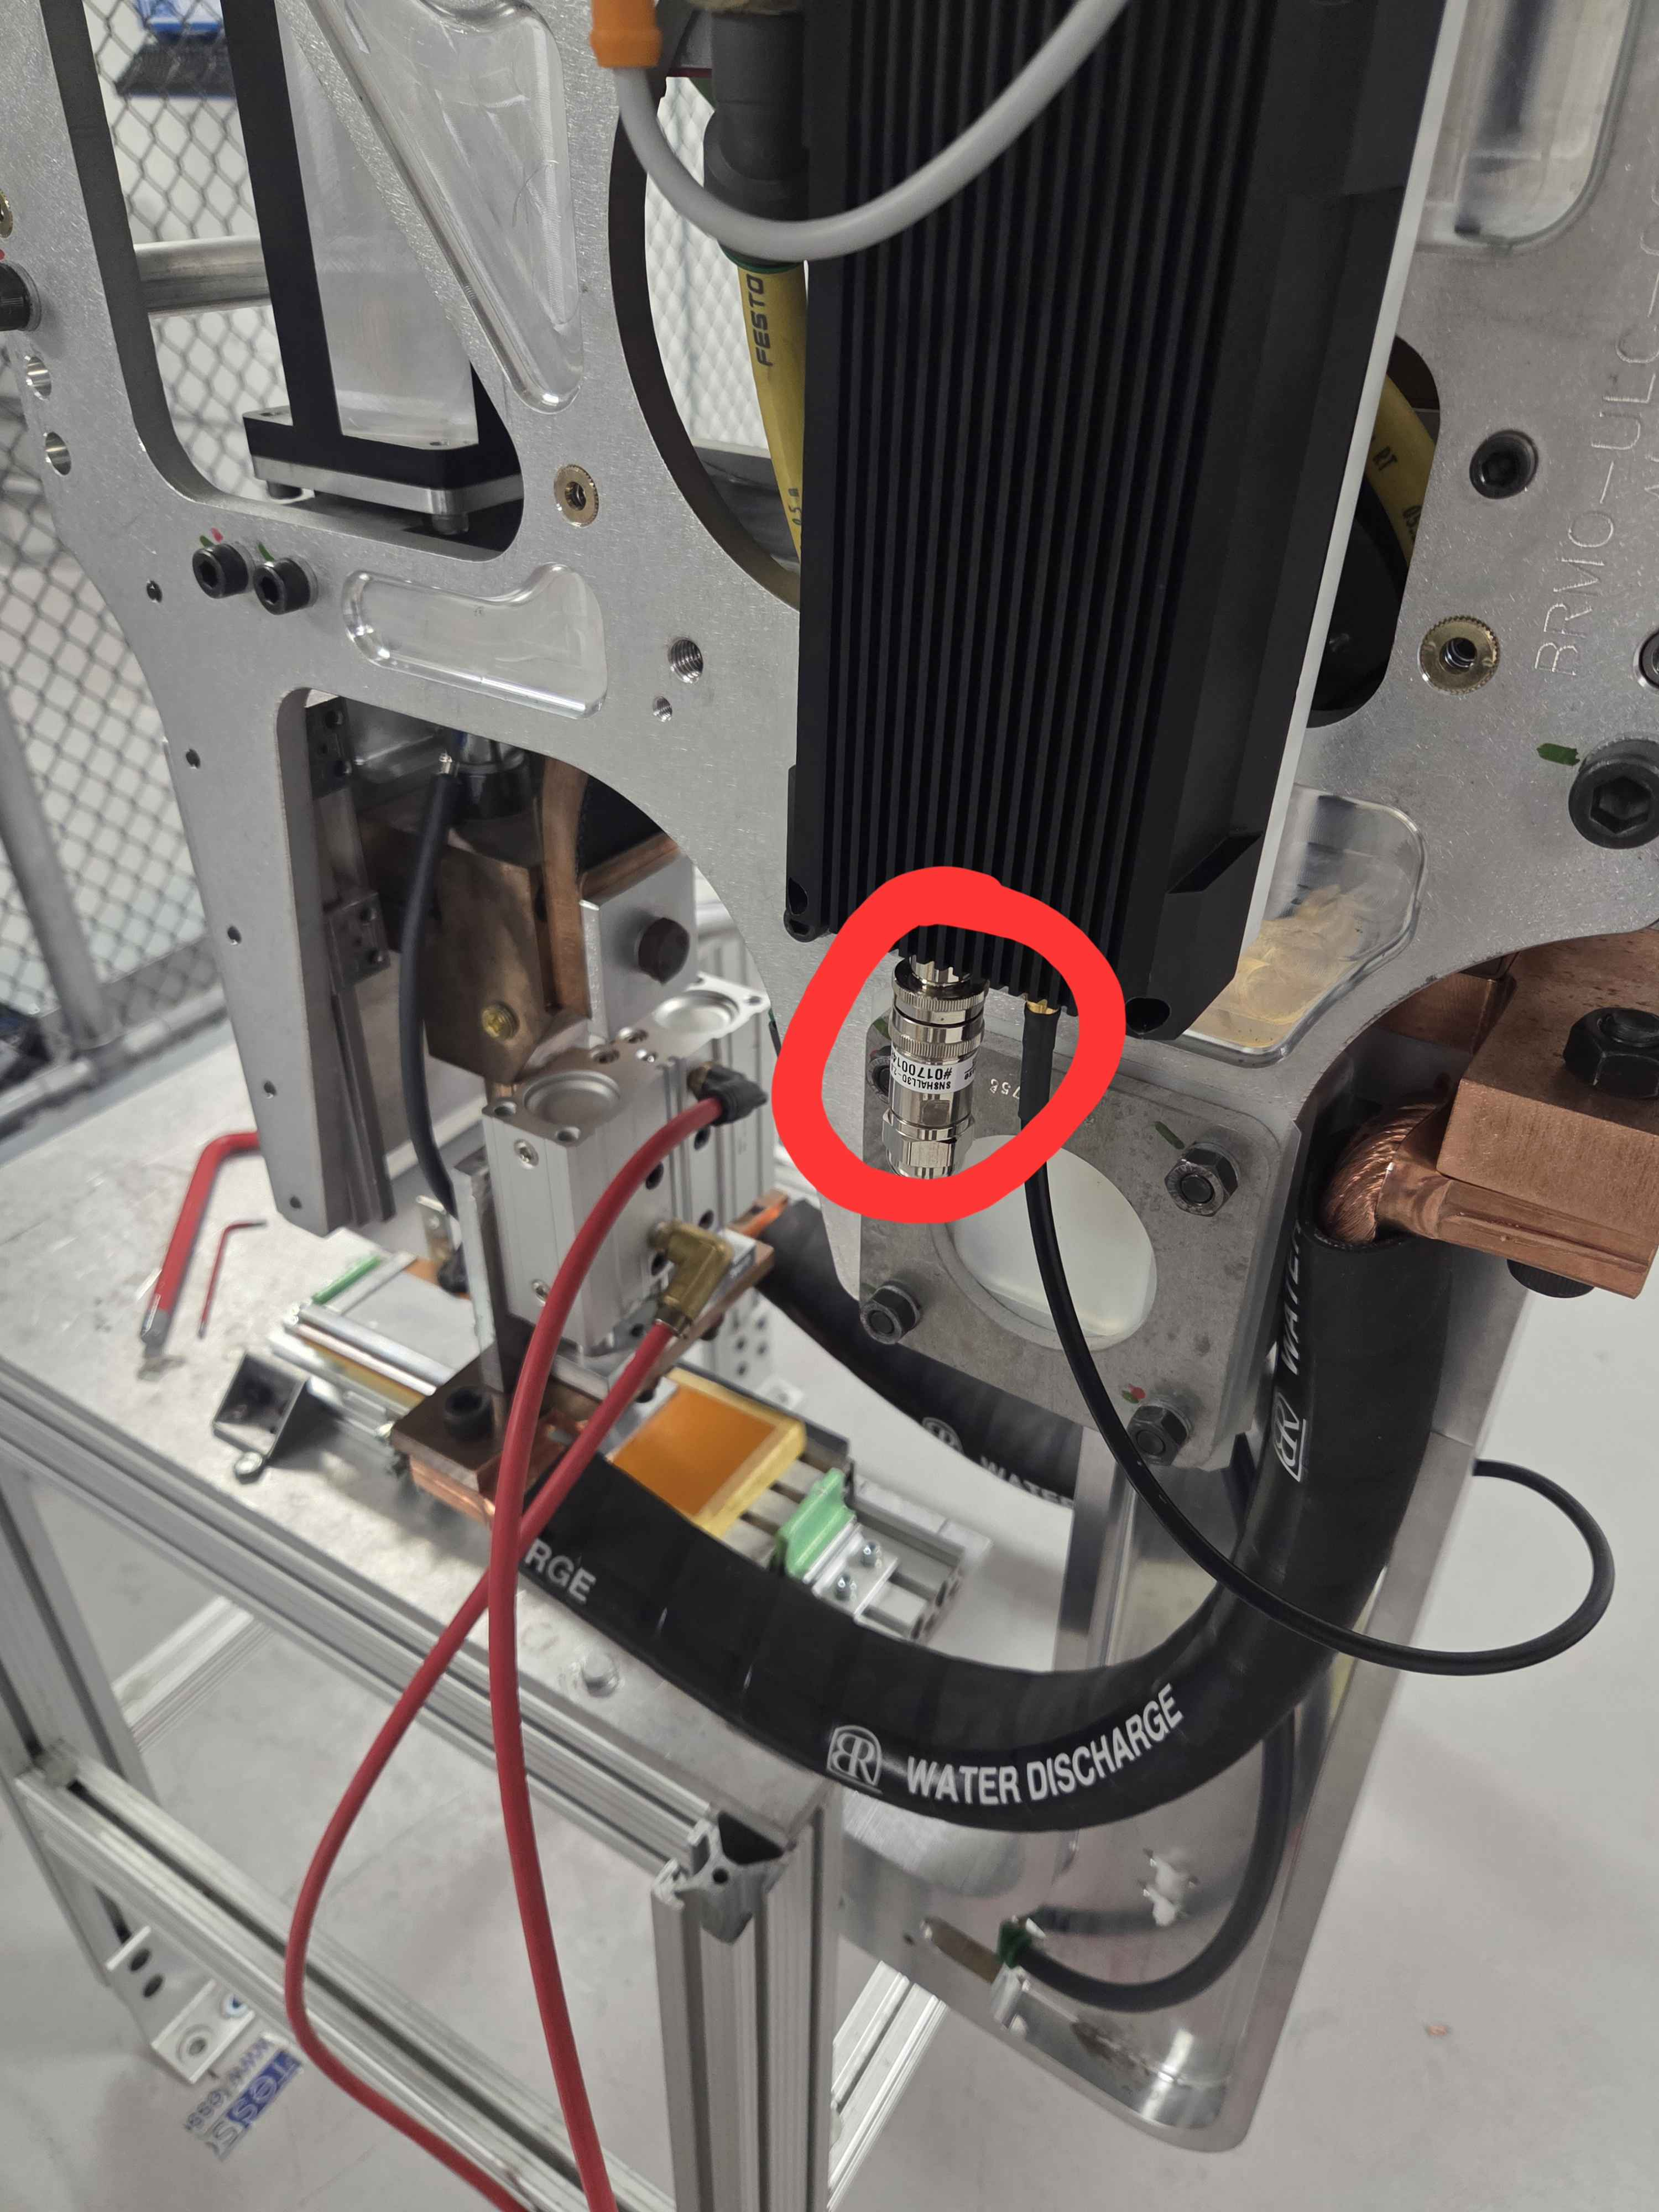
\includegraphics[width=\linewidth]{images/cylinder_hall.jpg}
                \end{subfigure}
                \hfill
                \begin{subfigure}{0.48\textwidth}
                    \centering
                    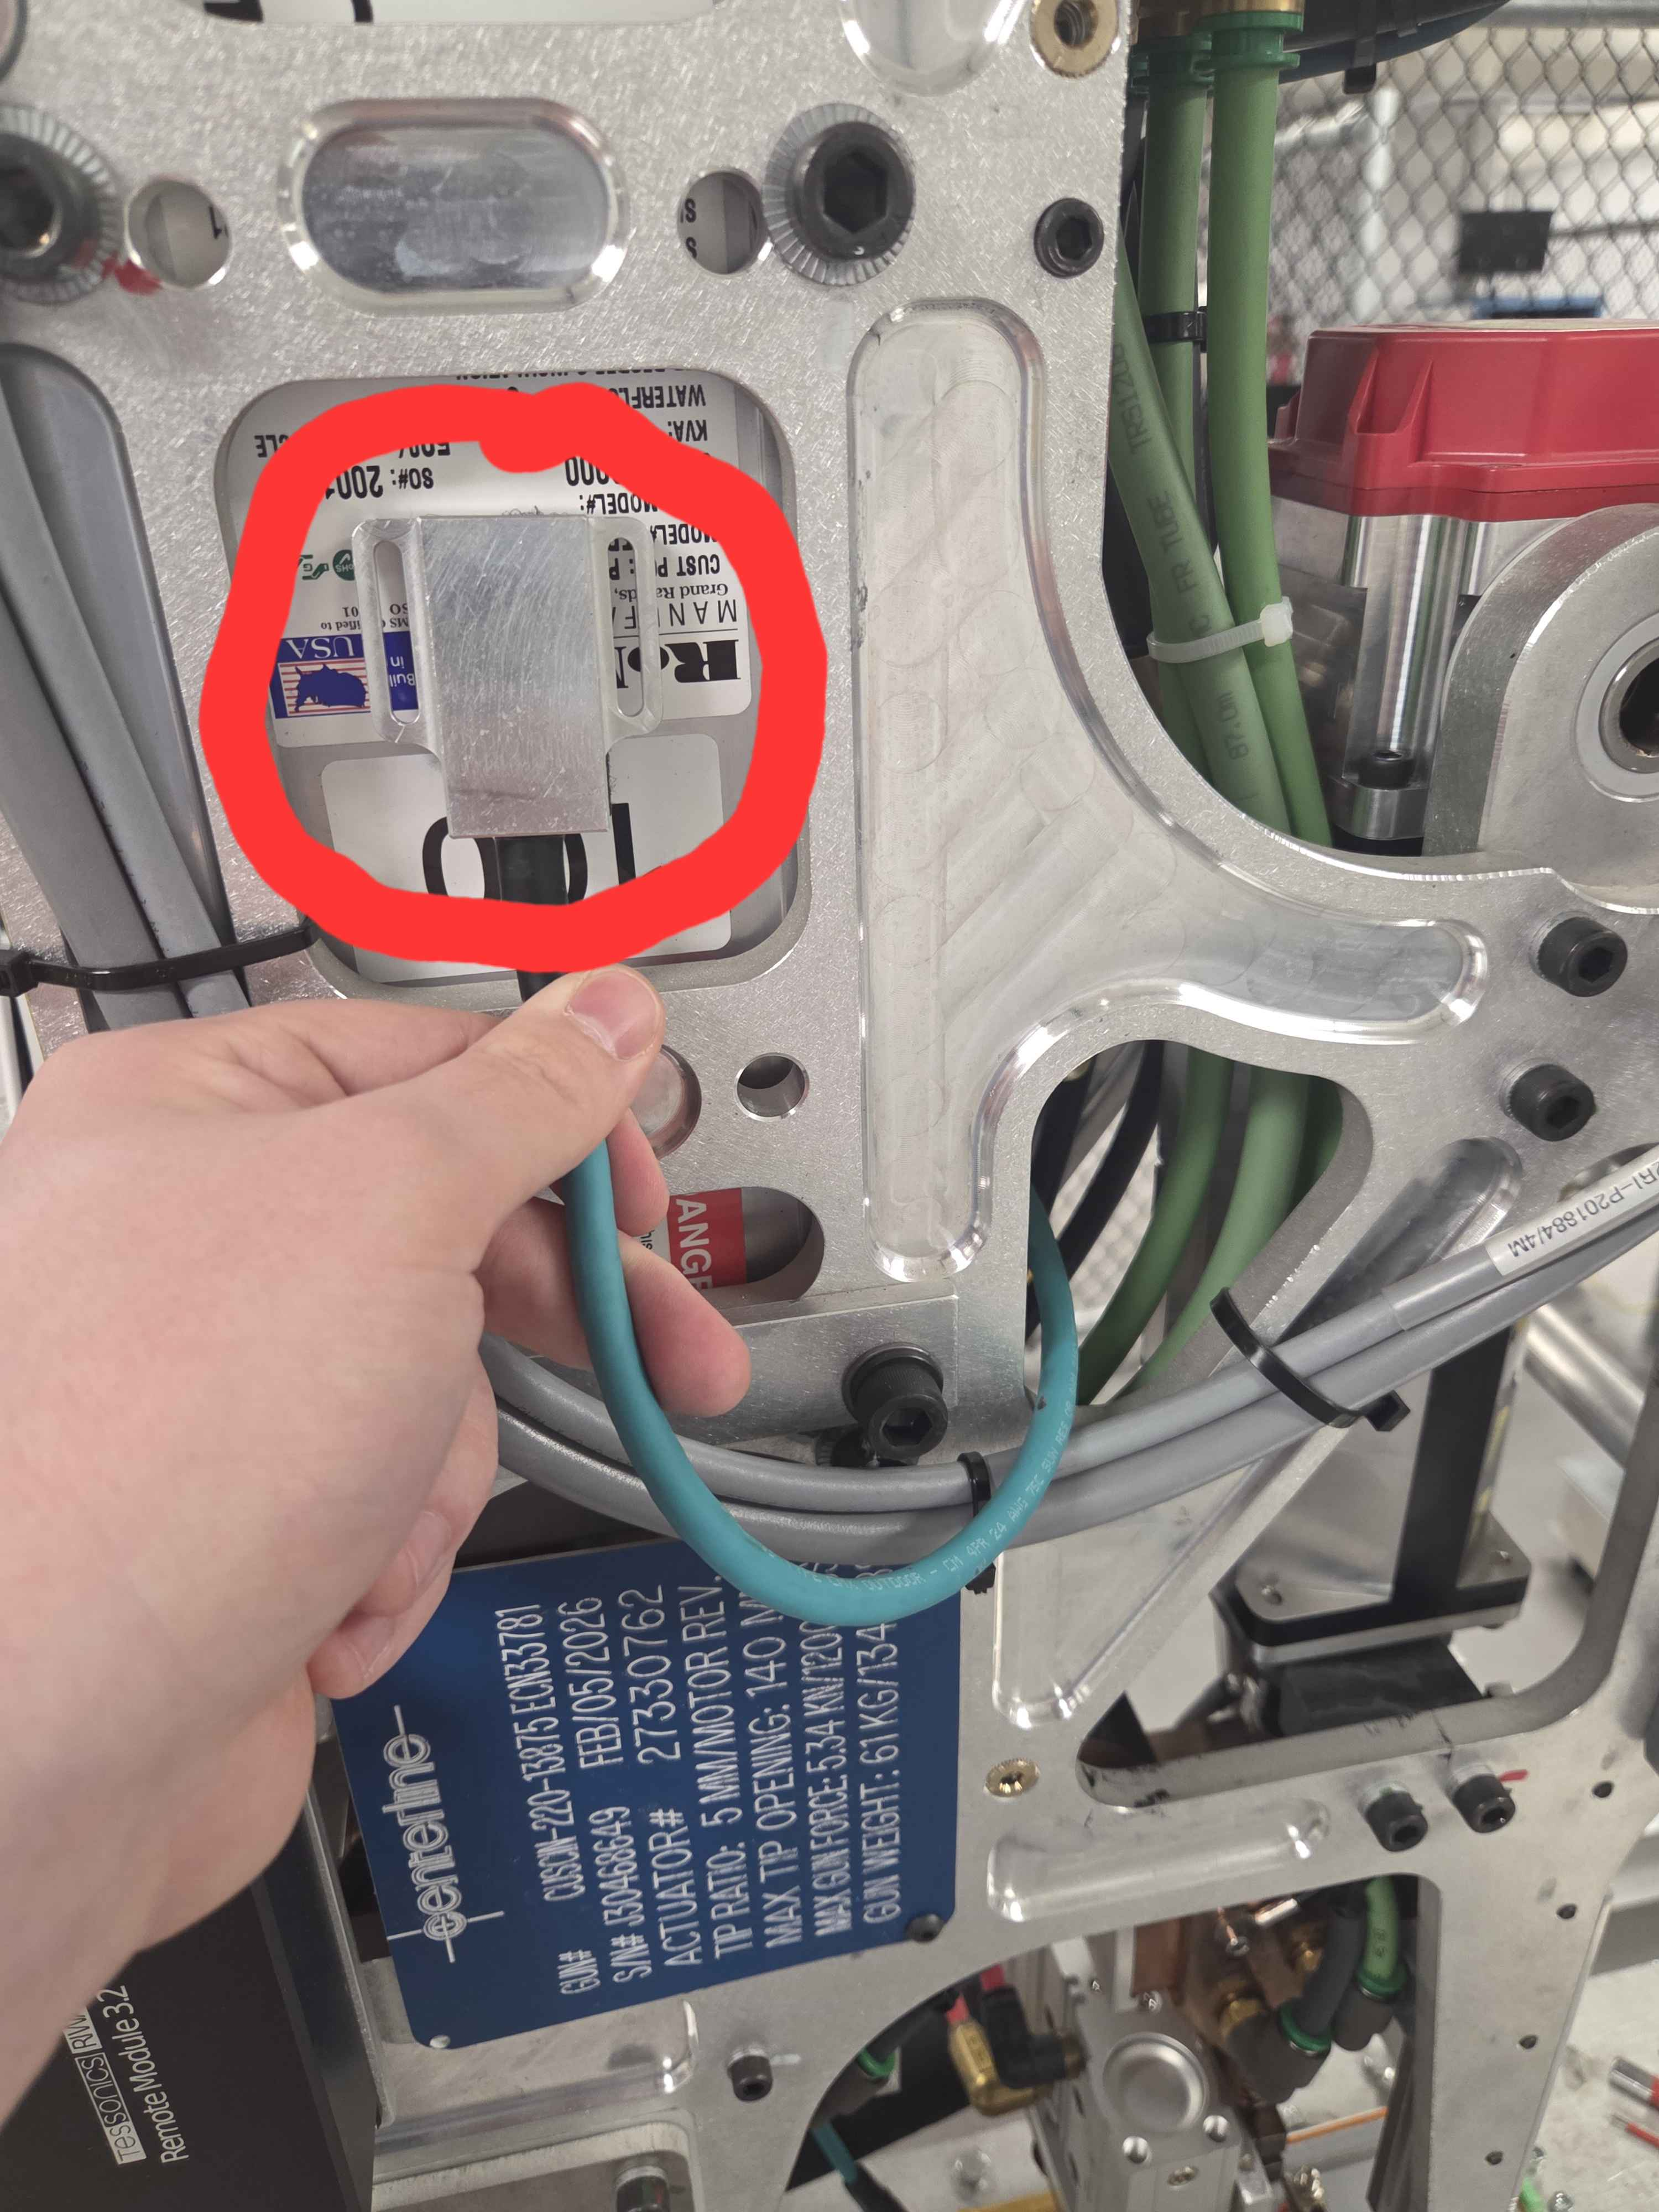
\includegraphics[width=\linewidth]{images/square_hall.jpg}
                \end{subfigure}
                \caption{Hall Effect Sensors installed on RSW Guns}
            \end{figure}
        \end{column}
    
    \end{columns}
\end{frame}


\begin{frame}{Algorithm Requirements}
    \begin{itemize}
        \item \textbf{Algorithm 1}: Filter out Hall Effect signal interference
        \begin{itemize}
            \item Real-time solution
            \item Small frame size to account for slower 1kHz acquisition frequency
            \item Minimal computational overhead to not disrupt main UPME processing 
        \end{itemize}
        \item \textbf{Algorithm 2}: Detect current on/off events
        \begin{itemize}
            \item Multi-impulse weld schedules
            \item Real-time UPME Constraints
        \end{itemize}
    \end{itemize}

    \begin{figure}
        \centering
        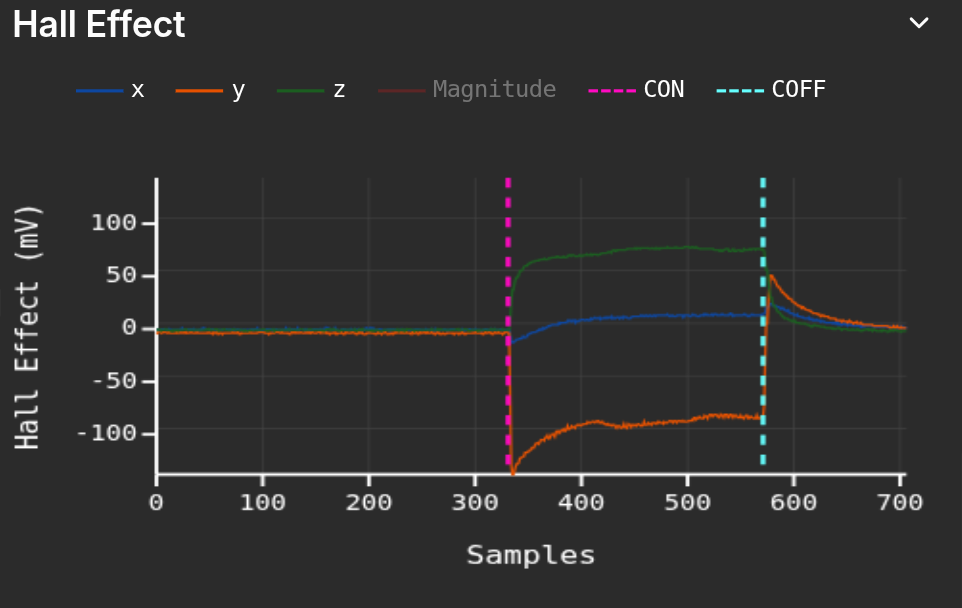
\includegraphics[width=0.5\linewidth]{images/hall_with_con.png}
        \caption{Denoised Hall Effect Signal from RSW Gun with Current Detected}
        \label{fig:hall_with_con}
    \end{figure}
\end{frame}
%------------------------------------------------
\begin{frame}{Problem Definition}
    \begin{columns}
        \begin{column}{0.4\textwidth}
            The Hall Effect sensor measurement at discrete sample index $n$ can be denoted as a discrete-time vector signal:
            \[
            \mathbf{Y}(n) = (x_n, y_n, z_n) \in \mathbb{R}^3,
            \]
            \[
            \mathbf{Y} : \mathbb{N} \rightarrow \mathbb{R}^3 
            \]
            where $x_n$, $y_n$, and $z_n$ are scalar measurements of the magnetic
            field components along the $x$, $y$, and $z$ axes at sample $n$
        \end{column}
        \begin{column}{0.6\textwidth}
            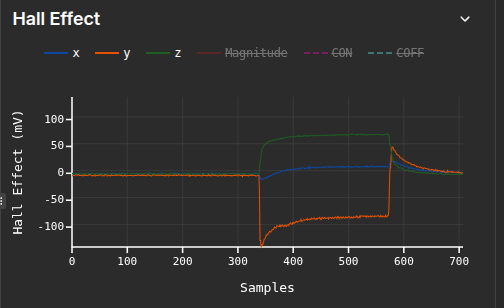
\includegraphics[width=\linewidth]{images/hall_effect_signal.png}
            \captionof{figure}{Hall Effect Signal from a RSW Gun}
        \end{column}
    \end{columns}
\end{frame}

%------------------------------------------------

\begin{frame}{Problem Definition}

We model the observed Hall signal as a superposition:

\[
\mathbf{Y}(n) = \sum_{i=1}^{K} \mathbf{X}_i(n) + \mathbf{N}(n)
\]

where

\[
\mathbf{X}_i(n) = (x_{i,n}, y_{i,n}, z_{i,n})
\]

represents the contribution from the $i$-th RSW Gun, and

\[
\mathbf{N}(n) = (x_{N,n}, y_{N,n}, z_{N,n})
\]

denotes residual noise not attributable to any distinct target source

\end{frame}

%------------------------------------------------

\begin{frame}{Problem Definition}
    Our goal is to recover the denoised signal of the target RSW gun that the sensor is physically installed on at sample index $n - m$, defined as:
    \[
    \hat{\mathbf{Y}}(n - m) = \mathbf{X}_{i^*}(n - m)
    \]
    
    where $i^* \in \{1, \ldots, K\}$ is the index of the source corresponding to the
    equipment on which the sensor is physically installed.
\end{frame}

%---------------------------------------------------------

\begin{frame}{Problem Definition}
We estimate the signal using a stateful algorithm relying on historically captured data for the observation window available at the current sample $n$:
\[
\left\{ \mathbf{Y}(j) \right\}_{j = \max(n - W_j + 1,\, 0)}^{\,n}
\]
where:
\begin{itemize}
    \item $W_j$ is the window length for the $j$-th lookup
    \item $m$ is a small \textit{look-ahead delay}, representing the number of samples collected \emph{after} the target sample before estimation is performed
\end{itemize}
\end{frame}

%------------------------------------------------
\begin{frame}{Problem Definition}
The parameter $m \ll W$ governs the \textbf{latency--accuracy trade-off}:
\begin{itemize}
    \item $m = 0$: zero-latency estimation
    \item $m > 0$: modest lookahead should permit improved source isolation at the cost of
    a fixed latency of $m$ samples
\end{itemize}
The objective is to find $\hat{\mathbf{Y}}(n-m)$ in \textbf{real-time}, with a minimal $m$ value

\vspace{0.5cm}

\begin{figure}[ht]
    \centering
    % --- Image row ---
    \begin{minipage}[c]{0.42\linewidth}
        \centering
        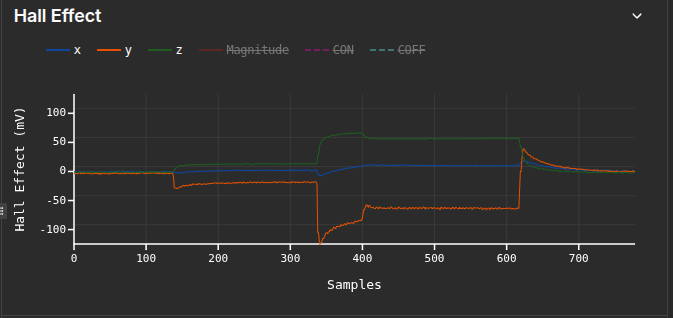
\includegraphics[width=\linewidth]{images/noisy_hall.png}
    \end{minipage}
    \hspace{0.02\linewidth}
    \begin{minipage}[c]{0.05\linewidth}
        \centering
        {\LARGE\textcolor{blue}{$\Rightarrow$}}
    \end{minipage}
    \hspace{0.02\linewidth}
    \begin{minipage}[c]{0.42\linewidth}
        \centering
        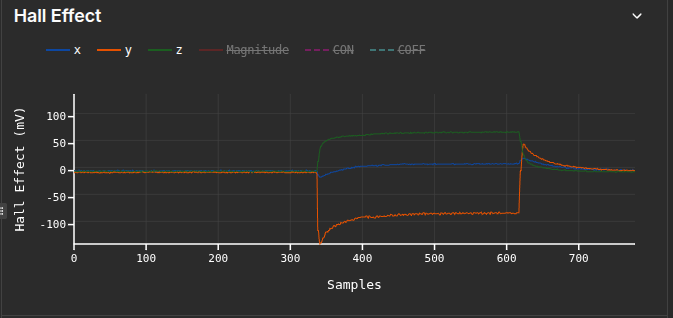
\includegraphics[width=\linewidth]{images/clean_hall.png}
    \end{minipage}

    % --- Caption row ---
    \begin{minipage}[t]{0.42\linewidth}
        \captionof{figure}{Noisy HES Signal, $K = 2$}
        \label{fig:noisy_hall}
    \end{minipage}
    \hspace{0.09\linewidth}
    \begin{minipage}[t]{0.42\linewidth}
        \captionof{figure}{Clean HES Signal, $\hat{\mathbf{Y}}(n)$}
        \label{fig:clean_hall}
    \end{minipage}
\end{figure}

\end{frame}

%------------------------------------------------
\section{Proposed Method}
\begin{frame}{Proposed Method - NEED HYPOTHESIS}
    \begin{itemize}
        \item Have an experiment already defined but need a method. I think \textbf{ICA} is promising here
        \item If I apply X method to my dataset then we should find $\hat{Y}(n)$
    \end{itemize}
\end{frame}
\subsection{Filtering Heuristic Algorithm}
\subsection{Current Detection Algorithm}
% -----------------------------------------------------------------------

\begin{frame}{Current Detection Algorithm Overview}
  \begin{block}{What it does}
    Identifies \textbf{Current~ON} (CON) and \textbf{Current~OFF} (COFF)
    transitions in a stream of Hall-effect magnitude samples using a
    dual-window sliding-median approach.
  \end{block}
  \vspace{0.5em}
  \begin{block}{How it works}
    \begin{itemize}
      \item Two windows of configurable size slide over the sample buffer.
      \item A statistically significant difference between window medians
            signals a state transition.
      \item Processing loops until a \textbf{weld end} condition is
            detected.
    \end{itemize}
  \end{block}
\end{frame}

%------------------------------------------------------------
\begin{frame}[fragile]{Call Graph}
  \begin{center}
  \begin{verbatim}
DetectCurrent  (iterates on new samples until weld end)
 +-- CurrentDetection
      +-- SetWindows
      +-- DetectChange
           +-- Median
           +-- StandardDeviation
           +-- if ChangeEvent
                +-- if PositiveChange
                    +-- CurrentOn
                +-- else
                    +-- CurrentOff
  \end{verbatim}
  \end{center}
\end{frame}

% -----------------------------------------------------------------------
\begin{frame}{Notation \& Configuration Parameters}
  \begin{columns}[T]
    
    \column{0.48\textwidth}
    \centering
    \captionof{table}{\textbf{Key Local Variables}}
    \scriptsize
    \begin{tabular}{cl}
      \hline
      \textbf{Symbol} & \textbf{Meaning} \\
      \hline
      $M$             & Magnitude sample buffer \\
      $E$             & Event list: $(i_\text{CON},\,i_\text{COFF})$ \\
      $\mathit{con}$  & \texttt{true} while current is ON \\
      $c_\text{off}$  & Post-COFF sample counter \\
      $w_e$           & Weld ended flag \\
      $\mathit{lw}$   & Left window \\
      $\mathit{rw}$   & Right window \\
      $\varnothing$   & Sentinel $= -1$ (not detected) \\
      \hline
    \end{tabular}

    \column{0.48\textwidth}
    \centering
    \captionof{table}{\textbf{Algorithm Input Params}}
    \scriptsize
    \begin{tabular}{crl}
      \hline
      \textbf{Param} & \textbf{Default} & \textbf{Role} \\
      \hline
      $W_S$ & 5  & \texttt{small\_window\_size} \\
      $W_L$ & 10  & \texttt{large\_window\_size} \\
      $\tau$ & 1.5 & Std-dev multiplier \\
      $T_e$ & 200 & Weld-end threshold \\
      $\sigma_\text{min}$ & 1.7 & Noise floor \\
      \hline
    \end{tabular}
  \end{columns}
\end{frame}

\begin{frame}{Main Loop --- DetectCurrent}
    \small
  \begin{algorithmic}[1]
    \Function{DetectCurrent}{$W_S,\, W_L,\, \tau,\, T_e,\, \sigma_\text{min}$}
      \State $M,E \gets [\,]$;\;
             $\mathit{con},w_e \gets \texttt{false}$;\;
             $c_\text{off} \gets 0$
      \While{$w_e = \texttt{false}$}
          \hfill\Comment{Iterates until weld end is detected}
        \State $M.\textsc{Append}\!\bigl(\|\textsc{GetNextCleanSample}()\|\bigr)$
        \If{$|M| > W_S + W_L$}
          \hfill\Comment{Start detection when windows are full}
          \If{$\lnot\mathit{con}$
              \textbf{ and } $|E|>0$}
            \State $c_\text{off} \gets c_\text{off} + 1$
          \EndIf
          \If{$\lnot w_e$ \textbf{ and } $c_\text{off} > T_e$}
            \State $w_e \gets \texttt{true}$
            \hfill\Comment{Weld end detected}
          \EndIf
          \State \Call{CurrentDetection}{$M,\, W_S,\, W_L,\, \tau,\, \sigma_\text{min},\, \mathit{con},\, E$}
        \EndIf
      \EndWhile
      \State \Return $E$
    \EndFunction
  \end{algorithmic}
\end{frame}

% -----------------------------------------------------------------------

\begin{frame}{Core Detection Step --- CurrentDetection}
  \begin{algorithmic}[1]
    \Function{CurrentDetection}{$M,\, W_S,\, W_L,\, \tau,\, \sigma_\text{min},\, \mathit{con},\, E$}
      \State $(\mathit{lw},\mathit{rw}) \gets \Call{SetWindows}{M,\, W_S,\, W_L,\, \mathit{con}}$
      \hfill\Comment{Left window, right window}
      \If{\Call{DetectChange}{$\mathit{lw},\,\mathit{rw},\,\tau,\,\sigma_\text{min}$}}
        \State \Call{ChangeEvent}{$\mathit{lw},\,\mathit{rw},\,M,\,\mathit{con},\,E$}
      \EndIf
    \EndFunction
  \end{algorithmic}
  \vspace{1em}
  \begin{block}{Three responsibilities}
    \begin{enumerate}
      \item Configure the two sliding windows.
      \item Detect a significant change between windows.
      \item Dispatch a state-change event if detected.
    \end{enumerate}
  \end{block}
\end{frame}

% -----------------------------------------------------------------------
\begin{frame}{Window Configuration --- SetWindows}
  \begin{columns}[T]
    \column{0.7\textwidth}
      \begin{algorithmic}[1]
        \Function{SetWindows}{$M,\, W_S,\, W_L,\, \mathit{con}$}
          \If{$\mathit{con}$ \textbf{(current ON)}}
            \State $\mathit{lw} \gets M[\,|M|{-}(W_S{+}W_L) : |M|{-}W_L\,)$
            \State $\mathit{rw} \gets M[\,|M|{-}W_L : |M|\,)$
          \Else
            \State $\mathit{lw} \gets M[\,|M|{-}(W_S{+}W_L) : |M|{-}W_S\,)$
            \State $\mathit{rw} \gets M[\,|M|{-}W_S : |M|\,)$
          \EndIf
          \State \Return $(\mathit{lw},\,\mathit{rw})$
        \EndFunction
      \end{algorithmic}

    \column{0.3\textwidth}
      \begin{block}{Key insight}
        Window sizes swap on state change so the larger context always
        covers the \emph{stable} (settled) region.
      \end{block}
      \vspace{0.5em}
      \begin{tabular}{lcc}
        \hline
        \textbf{State} & $|\mathit{lw}|$ & $|\mathit{rw}|$ \\
        \hline
        ON  & $W_S$ & $W_L$ \\
        OFF & $W_L$ & $W_S$ \\
        \hline
      \end{tabular}
  \end{columns}
\end{frame}

% -----------------------------------------------------------------------
\begin{frame}{Change Detection --- DetectChange}
  \begin{algorithmic}[1]
    \Function{DetectChange}{$\mathit{lw},\, \mathit{rw},\, \tau,\, \sigma_\text{min}$}
      \State $\delta \gets \bigl|\Call{Median}{\mathit{rw}} -
                                 \Call{Median}{\mathit{lw}}\bigr|$
      \State $\sigma_{lw} \gets \Call{StandardDeviation}{\mathit{lw},\, \sigma_\text{min}}$
      \State \Return $\delta > \tau \cdot \sigma_{lw}$
    \EndFunction
  \end{algorithmic}
  \vspace{1em}
  \begin{block}{Criterion}
    A change is \textbf{significant} when the absolute difference
    between window medians exceeds $\tau$ standard deviations of the
    left (reference) window. $\sigma_{lw}$ is clamped to $\sigma_\text{min}$, see \Call{StandardDeviation}{$w,\,\sigma_\text{min}$}.
  \end{block}
\end{frame}

% -----------------------------------------------------------------------

\begin{frame}{Event Dispatch --- ChangeEvent}
  \begin{algorithmic}[1]
    \Function{ChangeEvent}{$\mathit{lw},\, \mathit{rw},\, M,\, \mathit{con},\, E$}
      \State $\mathit{center} \gets |M| - |\mathit{rw}|$
      \hfill\Comment{Intersection index of the two windows}
      \If{$\Call{Median}{\mathit{rw}} > \Call{Median}{\mathit{lw}}$}
        \hfill\Comment{Change is positive}
        \If{$\lnot\mathit{con}$}
          \State \Call{CurrentOn}{$\mathit{center},\, \mathit{con},\, c_\text{off},\, E$}
          \hfill\Comment{OFF $\to$ ON}
        \EndIf
      \Else
        \If{$\mathit{con}$}
          \State \Call{CurrentOff}{$\mathit{center},\, \mathit{con},\, E$}
          \hfill\Comment{ON $\to$ OFF}
        \EndIf
      \EndIf
    \EndFunction
  \end{algorithmic}
\end{frame}

\begin{frame}{Event Recording --- CurrentOn / CurrentOff}
  \begin{columns}[T]
    % Left column: stacked functions
    \column{0.7\textwidth}
      \begin{block}{CurrentOn($i,\; \mathit{con},\; c_\text{off},\; E$)}
        \begin{algorithmic}[1]
          \Function{CurrentOn}{$i,\, \mathit{con},\, c_\text{off},\, E$}
            \State $E.\textsc{Append}((i,\,\varnothing))$
            \State $\mathit{con} \gets \texttt{true}$
            \State $c_\text{off} \gets 0$
          \EndFunction
        \end{algorithmic}
      \end{block}
      \vspace{0.8em}
      \begin{block}{CurrentOff($i,\; \mathit{con},\; E$)}
        \begin{algorithmic}[1]
          \Function{CurrentOff}{$i,\, \mathit{con},\, E$}
            \State $E.\text{last}.\mathit{COFF} \gets i$
            \State $\mathit{con} \gets \texttt{false}$
          \EndFunction
        \end{algorithmic}
      \end{block}

    % Right column: invariant
    \column{0.25\textwidth}
        \centering
      \begin{alertblock}{Important Note}
        Every CON event is eventually paired with exactly one COFF event.
        The sentinel $\varnothing = -1$ marks an unpaired CON event.
      \end{alertblock}
  \end{columns}
\end{frame}

\begin{frame}{Window Statistics --- Median \& Standard Deviation}
  \begin{columns}[T]
    \column{0.38\textwidth}
      \begin{block}{Median($w$)}
        \begin{algorithmic}[1]
          \Function{Median}{$w$}
            \State $A \gets \textsc{Copy}(w)$
            \State Partial-sort $A$ at $\lfloor n/2 \rfloor$
            \State \Return $A[\lfloor n/2 \rfloor]$
          \EndFunction
        \end{algorithmic}
      \end{block}

    \column{0.55\textwidth}
      \begin{block}{StandardDeviation($w,\; \sigma_\text{min}$)}
        \begin{algorithmic}[1]
          \Function{StandardDeviation}{$w,\, \sigma_\text{min}$}
            \State $\mu \gets \frac{1}{n}\sum_{x \in w} x$
            \State $\sigma \gets \sqrt{\frac{1}{n}\sum_{x \in w}(x-\mu)^2}$
            \If{$\sigma < \sigma_\text{min}$}
              \State $\sigma \gets \sigma_\text{min}$
            \EndIf
            \State \Return $\sigma$
          \EndFunction
        \end{algorithmic}
      \end{block}
  \end{columns}
  \vspace{0.5em}
  \begin{block}{Note on noise floor}
    Standard deviation is clamped to $\sigma_\text{min} = 1.7$ to
    prevent false positives on near-constant signal segments.
  \end{block}
\end{frame}

% -----------------------------------------------------------------------
\begin{frame}{Summary of Current Detection Algorithm}
  \begin{enumerate}
    \item \textbf{DetectCurrent} loops, consuming one sample per iteration,
          until the weld-end counter $c_\text{off}$ exceeds $T_e$.
    \item Each iteration runs \textbf{CurrentDetection}:
          configures windows, records stats, checks for change.
    \item \textbf{SetWindows} swaps window sizes based on current state
          to keep the stable region in the larger window.
    \item \textbf{DetectChange} uses a median-delta vs.\ std-dev test
          ($\delta > \tau\sigma_{lw}$) for robustness to noise.
    \item \textbf{ChangeEvent} dispatches \textbf{CurrentOn} or
          \textbf{CurrentOff} based on direction of change.
    \item Results are returned as a list of
          $(i_\text{CON},\,i_\text{COFF})$ index pairs.
  \end{enumerate}
\end{frame}
%------------------------------------------------
\section{Timeline}
\begin{frame}{Research Timeline}
\small
\begin{tabular}{p{2.5cm} p{8cm}}
\hline
\textbf{Date} & \textbf{Milestone / Tasks} \\
\hline
Apr 10 & Proposal Presentation \\

Apr 11 -- Apr 30 & Data pipeline, synthetic data generation \\

May 1 -- May 15 & Implement baseline methods (LMS, filters), initial evaluation \\

May 16 -- Jun 5 & Develop proposed heuristic algorithm, parameter tuning \\

Jun 6 -- Jun 25 & Experimental evaluation, robustness analysis, comparisons \\

Jun 26 -- Jul 10 & Thesis writing, figures, results consolidation \\

Jul 11 -- Jul 25 & Revision, refinement, additional experiments (if needed) \\

Jul 26 -- Jul 31 & Defense preparation (slides, rehearsal, final edits) \\
\hline
\end{tabular}

\vspace{0.5cm}
\centering
\textbf{Target Defense: Early August 2026}
\end{frame}
%---------------------------------------------------------
\section{References}

\begin{frame}[allowframebreaks]{References}
    \bibliographystyle{IEEEtran}
    \bibliography{references}
\end{frame}

%------------------------------------------------
\begin{frame}
    \centering
    \Huge Thank You
\end{frame}

\end{document}
